\documentclass{standalone}
\usepackage{tikz}
\usetikzlibrary{patterns, positioning}


\begin{document}
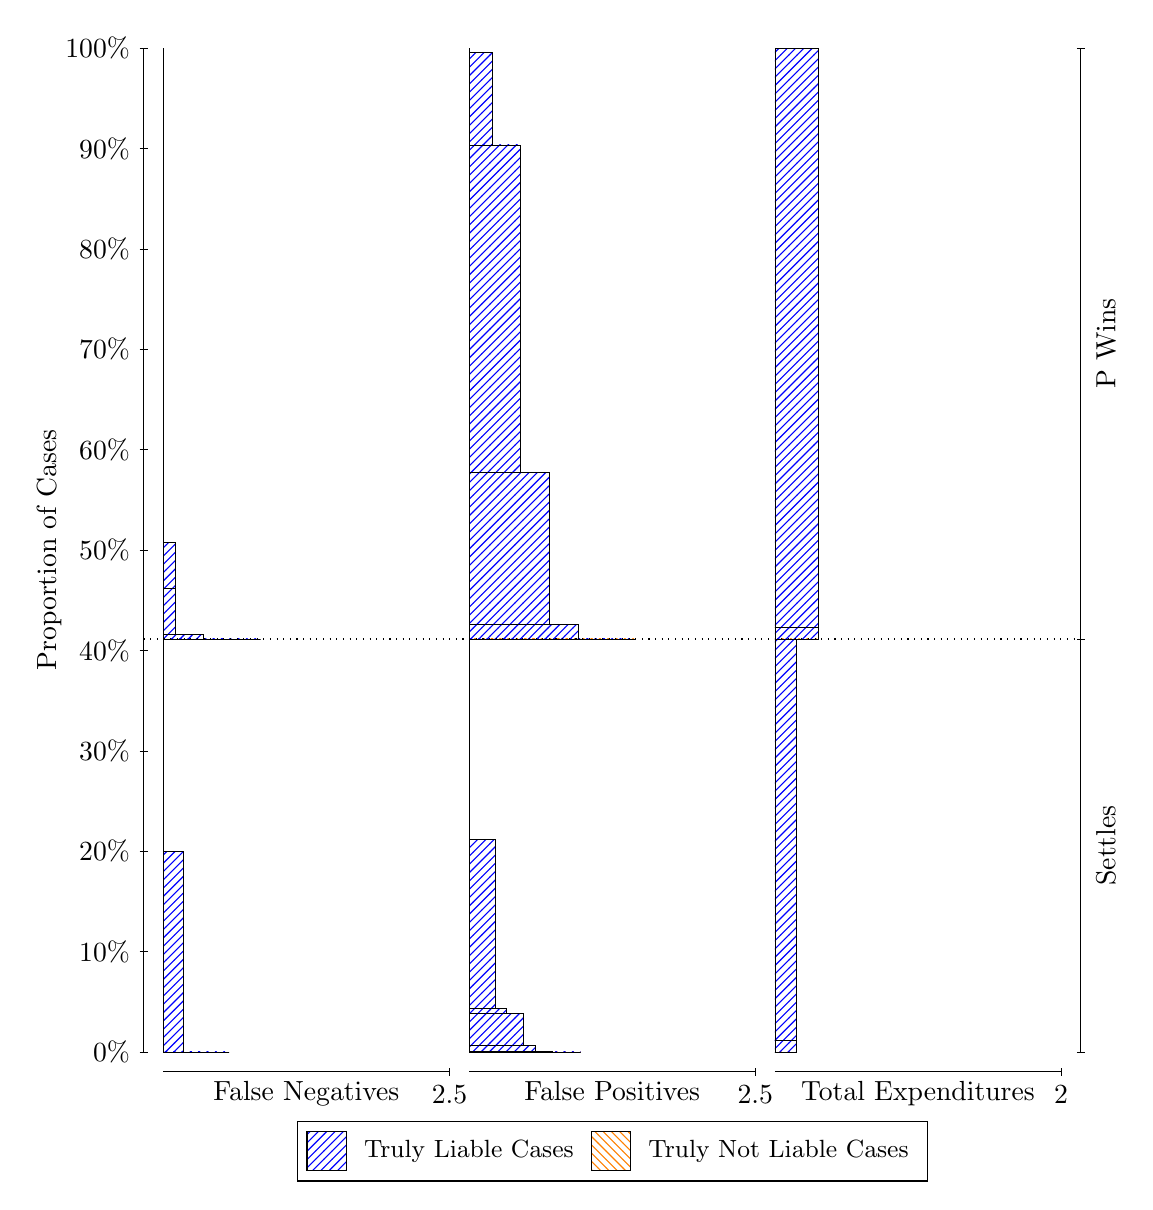
\begin{tikzpicture}
\draw[black, very thin] (1.5,1.75) -- (1.5,14.5);
\node[rotate=90, text=black, anchor=center] at (0.3, 8.125) {Proportion of Cases};
\draw[black, very thin] (1.45,1.75) -- (1.55,1.75);
\node[text=black, anchor=east] at (1.45, 1.75) {0\%};
\draw[black, very thin] (1.45,3.025) -- (1.55,3.025);
\node[text=black, anchor=east] at (1.45, 3.025) {10\%};
\draw[black, very thin] (1.45,4.3) -- (1.55,4.3);
\node[text=black, anchor=east] at (1.45, 4.3) {20\%};
\draw[black, very thin] (1.45,5.575) -- (1.55,5.575);
\node[text=black, anchor=east] at (1.45, 5.575) {30\%};
\draw[black, very thin] (1.45,6.85) -- (1.55,6.85);
\node[text=black, anchor=east] at (1.45, 6.85) {40\%};
\draw[black, very thin] (1.45,8.125) -- (1.55,8.125);
\node[text=black, anchor=east] at (1.45, 8.125) {50\%};
\draw[black, very thin] (1.45,9.4) -- (1.55,9.4);
\node[text=black, anchor=east] at (1.45, 9.4) {60\%};
\draw[black, very thin] (1.45,10.675) -- (1.55,10.675);
\node[text=black, anchor=east] at (1.45, 10.675) {70\%};
\draw[black, very thin] (1.45,11.95) -- (1.55,11.95);
\node[text=black, anchor=east] at (1.45, 11.95) {80\%};
\draw[black, very thin] (1.45,13.225) -- (1.55,13.225);
\node[text=black, anchor=east] at (1.45, 13.225) {90\%};
\draw[black, very thin] (1.45,14.5) -- (1.55,14.5);
\node[text=black, anchor=east] at (1.45, 14.5) {100\%};

\draw[black, very thin] (13.4,1.75) -- (13.4,14.5);
\draw[black, very thin] (13.35,1.75) -- (13.45,1.75);
\node[anchor=west] at (13.35, 1.75) {};
\draw[black, very thin] (13.35,6.995) -- (13.45,6.995);
\node[anchor=west] at (13.35, 6.995) {};
\draw[black, very thin] (13.35,14.5) -- (13.45,14.5);
\node[anchor=west] at (13.35, 14.5) {};

\draw[black, very thin, pattern color=blue, pattern=north east lines] (1.75,1.75) rectangle (2.5857,1.75);
\draw[black, very thin, pattern color=blue, pattern=north east lines] (1.75,1.75) rectangle (2.295,1.75);
\draw[black, very thin, pattern color=blue, pattern=north east lines] (1.75,1.75) rectangle (2.2223,1.75);
\draw[black, very thin, pattern color=blue, pattern=north east lines] (1.75,1.75) rectangle (2.0043,4.2958);
\draw[black, very thin, pattern color=blue, pattern=north east lines] (1.75,4.2958) rectangle (1.9317,4.2958);
\draw[black, very thin, pattern color=blue, pattern=north east lines] (1.75,4.2958) rectangle (1.859,4.2964);
\draw[black, very thin, pattern color=orange, pattern=north west lines] (1.75,4.2964) rectangle (1.75,4.2964);
\draw[black, very thin, pattern color=blue, pattern=north east lines] (1.75,4.2964) rectangle (1.75,6.995);
\draw[black, very thin, pattern color=blue, pattern=north east lines] (1.75,6.995) rectangle (2.9853,6.995);
\draw[black, very thin, pattern color=blue, pattern=north east lines] (1.75,6.995) rectangle (2.622,6.9951);
\draw[black, very thin, pattern color=blue, pattern=north east lines] (1.75,6.9951) rectangle (2.2587,7.0524);
\draw[black, very thin, pattern color=blue, pattern=north east lines] (1.75,7.0524) rectangle (1.8953,7.6352);
\draw[black, very thin, pattern color=blue, pattern=north east lines] (1.75,7.6352) rectangle (1.8953,8.2249);
\draw[black, very thin, pattern color=orange, pattern=north west lines] (1.75,8.2249) rectangle (1.75,8.2249);
\draw[black, very thin, pattern color=blue, pattern=north east lines] (1.75,8.2249) rectangle (1.75,14.5);
\draw[black, very thin, pattern color=orange, pattern=north west lines] (5.6333,1.75) rectangle (7.0503,1.75);
\draw[black, very thin, pattern color=blue, pattern=north east lines] (5.6333,1.75) rectangle (7.0503,1.75);
\draw[black, very thin, pattern color=orange, pattern=north west lines] (5.6333,1.75) rectangle (6.7597,1.75);
\draw[black, very thin, pattern color=blue, pattern=north east lines] (5.6333,1.75) rectangle (6.7597,1.75);
\draw[black, very thin, pattern color=blue, pattern=north east lines] (5.6333,1.75) rectangle (6.687,1.7533);
\draw[black, very thin, pattern color=orange, pattern=north west lines] (5.6333,1.7533) rectangle (6.469,1.7533);
\draw[black, very thin, pattern color=blue, pattern=north east lines] (5.6333,1.7533) rectangle (6.469,1.8314);
\draw[black, very thin, pattern color=blue, pattern=north east lines] (5.6333,1.8314) rectangle (6.3963,1.8315);
\draw[black, very thin, pattern color=blue, pattern=north east lines] (5.6333,1.8315) rectangle (6.3237,2.236);
\draw[black, very thin, pattern color=blue, pattern=north east lines] (5.6333,2.236) rectangle (6.1057,2.3035);
\draw[black, very thin, pattern color=blue, pattern=north east lines] (5.6333,2.3035) rectangle (6.033,2.3037);
\draw[black, very thin, pattern color=blue, pattern=north east lines] (5.6333,2.3037) rectangle (5.9603,4.4486);
\draw[black, very thin, pattern color=blue, pattern=north east lines] (5.6333,4.4486) rectangle (5.7423,4.4491);
\draw[black, very thin, pattern color=blue, pattern=north east lines] (5.6333,4.4491) rectangle (5.6697,4.4491);
\draw[black, very thin, pattern color=blue, pattern=north east lines] (5.6333,4.4491) rectangle (5.6333,6.995);
\draw[black, very thin, pattern color=orange, pattern=north west lines] (5.6333,6.995) rectangle (7.7407,6.995);
\draw[black, very thin, pattern color=blue, pattern=north east lines] (5.6333,6.995) rectangle (7.7407,6.995);
\draw[black, very thin, pattern color=orange, pattern=north west lines] (5.6333,6.995) rectangle (7.3773,6.995);
\draw[black, very thin, pattern color=blue, pattern=north east lines] (5.6333,6.995) rectangle (7.3773,6.9975);
\draw[black, very thin, pattern color=orange, pattern=north west lines] (5.6333,6.9975) rectangle (7.014,6.9975);
\draw[black, very thin, pattern color=blue, pattern=north east lines] (5.6333,6.9975) rectangle (7.014,7.1758);
\draw[black, very thin, pattern color=orange, pattern=north west lines] (5.6333,7.1758) rectangle (6.6507,7.1758);
\draw[black, very thin, pattern color=blue, pattern=north east lines] (5.6333,7.1758) rectangle (6.6507,9.1068);
\draw[black, very thin, pattern color=orange, pattern=north west lines] (5.6333,9.1068) rectangle (6.2873,9.1068);
\draw[black, very thin, pattern color=blue, pattern=north east lines] (5.6333,9.1068) rectangle (6.2873,13.27);
\draw[black, very thin, pattern color=blue, pattern=north east lines] (5.6333,13.27) rectangle (5.924,14.443);
\draw[black, very thin, pattern color=blue, pattern=north east lines] (5.6333,14.443) rectangle (5.6333,14.5);
\draw[black, very thin, pattern color=orange, pattern=north west lines] (9.5167,1.75) rectangle (9.7892,1.75);
\draw[black, very thin, pattern color=blue, pattern=north east lines] (9.5167,1.75) rectangle (9.7892,1.8962);
\draw[black, very thin, pattern color=orange, pattern=north west lines] (9.5167,1.8962) rectangle (9.7892,1.8962);
\draw[black, very thin, pattern color=blue, pattern=north east lines] (9.5167,1.8962) rectangle (9.7892,6.995);
\draw[black, very thin, pattern color=orange, pattern=north west lines] (9.5167,6.995) rectangle (10.062,6.995);
\draw[black, very thin, pattern color=blue, pattern=north east lines] (9.5167,6.995) rectangle (10.062,7.1419);
\draw[black, very thin, pattern color=orange, pattern=north west lines] (9.5167,7.1419) rectangle (10.062,7.1419);
\draw[black, very thin, pattern color=blue, pattern=north east lines] (9.5167,7.1419) rectangle (10.062,14.5);
\draw[black, dotted] (1.5,6.995) -- (13.4,6.995);
\draw[black, very thin] (1.75,1.5) -- (5.3833,1.5);
\node[text=black, anchor=north] at (3.5667, 1.5) {False Negatives};
\draw[black, very thin] (5.3833,1.45) -- (5.3833,1.55);
\node[text=black, anchor=north] at (5.3833, 1.45) {2.5};

\draw[black, very thin] (5.6333,1.5) -- (9.2667,1.5);
\node[text=black, anchor=north] at (7.45, 1.5) {False Positives};
\draw[black, very thin] (9.2667,1.45) -- (9.2667,1.55);
\node[text=black, anchor=north] at (9.2667, 1.45) {2.5};

\draw[black, very thin] (9.5167,1.5) -- (13.15,1.5);
\node[text=black, anchor=north] at (11.333, 1.5) {Total Expenditures};
\draw[black, very thin] (13.15,1.45) -- (13.15,1.55);
\node[text=black, anchor=north] at (13.15, 1.45) {2};

\node[text=black, centered, rotate=90] at (13.72, 4.3725) {Settles};
\node[text=black, centered, rotate=90] at (13.72, 10.747) {P Wins};

\draw (7.449999999999999,1.5) node[draw=none] (baseCoordinate) {};
\begin{scope}[align=center]
        \matrix[scale=0.5, draw=black, below=0.5cm of baseCoordinate, nodes={draw}, column sep=0.1cm]{
            \node[rectangle, draw, minimum width=0.5cm, minimum height=0.5cm, pattern color=blue, pattern=north east lines] {}; &
            \node[draw=none, font=\small, text=black] (B) {Truly Liable Cases}; &
            \node[rectangle, draw, minimum width=0.5cm, minimum height=0.5cm, pattern color=orange, pattern=north west lines] {}; &
            \node[draw=none, font=\small, text=black] (B) {Truly Not Liable Cases}; \\
            };
\end{scope}

\end{tikzpicture}
\end{document}